\chapter{Feasibility Study}

\quad  In this appendix, we discuss the feasibility of C4IAN. 
As chapter \ref{ch:feasability} covered marketing and financial aspects, we will focus on technical, operational, and legal feasibility.

\section{Technical Feasibility}

\quad To design C4IAN, a strong background in networks is required, especially mobile ad-hoc networks. The resources for learning networks are abundant, but those for mobile ad-hoc networks are scarce. Learning about routing in mobile ad-hoc networks and choosing adequate protocols to implement is not an easy task.

After the produce is designed, the implementation phase requires skills in low level programming. As the router module interfaces extensively with the Linux kernel, and it's network stack, knowledge about low level programming and networks programming is a must. Since the Linux kernel is open source, the implementation could be completed without major obstacles. The router could be implemented in user mode, or as a kernel module. Both are available options due to the flexibility of the Linux kernel. As Linux is a relatively lightweight operating system that can be deployed on various hardware, deploying C4IAN on most types of hardware should not be problematic.

\section{Operational Feasibility}

\quad From the user's point of view, C4IAN is a very easy system to operate. Most of the complexity is hidden in the router implementation, which the users (and the applications) do not directly interact with. The router module interacts exclusively with the Linux kernel. From the perspective of a user, or an application developer, the system is transparent. The implementation of applications is not affected by the design or implementation of the router. This gives a lot of flexibility for developers working on producing applications that utilize the routing capabilities offered by C4IAN. As for the command center and unit applications provided by C4IAN, they are very straightforward to deal with. They provide a simple interface for users to send and receive messages through simple GUIs. This is explained further in \ref{sec:usage}.

\section{Legal Feasibility}

\quad C4IAN strictly uses open source packages in its development, so the usage and distribution of C4IAN and its code should not cause any legal troubles.

In our initial design of C4IAN, we use Wi-Fi as the MAC Layer. This causes no legal problems as Wi-Fi bands belong to the ISM bands, which are free to use without licensing. For some applications, a different band with different properties may be required. Even though the router implementation mostly will not need to be modified to accommodate other MAC layers, some legal obstacles may rise. Using bands outside the ISM bands requires legal licensing, with laws differing by country. If C4IAN is to be operated in such bands, necessary licensing must be acquired first.

\section{SWOT Analysis}
Figure \ref{fig:swot} shows the SWOT (Strengths, Weaknesses, Opportunities and Threats) analysis of the product.
SWOT analysis helps in project and expectations management.

One of the main weaknesses of the product is that it only targets Linux.
However, it is not a major problem, as at the end the product will be installed on closed embedded systems and mostly users will be indifferent.

The product is user-friendly and scalable, yet the customers have difficult requirements.

\begin{figure}[!htb]
    \centering
    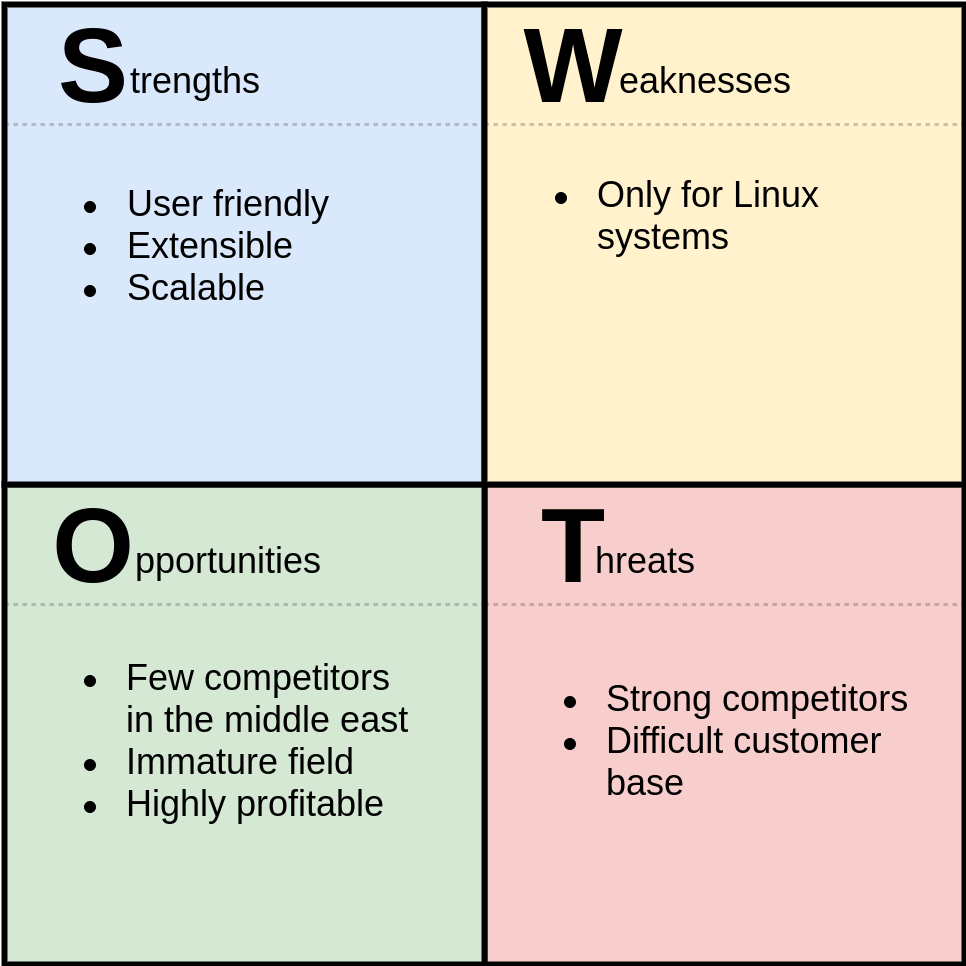
\includegraphics[width=0.6\linewidth]{images/swot.png}
    \caption{SWOT Analysis}
    \label{fig:swot}
\end{figure}